
\documentclass{beamer}

% For more themes, color themes and font themes, see:
% http://deic.uab.es/~iblanes/beamer_gallery/index_by_theme.html
%
\mode<presentation>
{
  \usetheme{Madrid}       % or try default, Darmstadt, Warsaw, ...
  \usecolortheme{default} % or try albatross, beaver, crane, ...
  \usefonttheme{serif}    % or try default, structurebold, ...
  \setbeamertemplate{navigation symbols}{}
  \setbeamertemplate{caption}[numbered]
} 

\usepackage[english]{babel}
\usepackage[utf8x]{inputenc}
\usepackage{chemfig}
\usepackage[version=3]{mhchem}

% On Overleaf, these lines give you sharper preview images.
% You might want to `comment them out before you export, though.
\usepackage{pgfpages}
\pgfpagesuselayout{resize to}[%
  physical paper width=8in, physical paper height=6in]

% Here's where the presentation starts, with the info for the title slide
\title[Java Tutorial  \Talentio]{Java Tutorial}
\author{Mohammad Imtiaz}
\institute{}
\date{\today}

\begin{document}

\begin{frame}
  \titlepage
\end{frame}

% These three lines create an automatically generated table of contents.
\begin{frame}{What is Java?}
 \begin{itemize}
 \item Java is a high-level programming language originally developed by Sun Microsystems and released in 1995. Java runs on a variety of platforms, such as Windows, Mac OS, and the various versions of UNIX. 
 \end{itemize}
\end{frame}

\begin{frame}{Prerequisites}
	\begin{itemize}
	\item 	Before you start practicing various types of examples given in this reference, we assume that you are already aware about computer programs and computer programming languages.

	\end{itemize}
\end{frame}

% Java Overview and History.

\begin{frame}{History}
	\begin{itemize}
	\item 	Java programming language was originally developed by Sun Microsystems which was initiated by James Gosling and released in 1995 as core component of Sun Microsystems' Java platform (Java 1.0 [J2SE]).
	
\begin{itemize}
\item The latest release of the Java Standard Edition is Java SE 8. With the advancement of Java and its widespread popularity, multiple configurations were built to suit various types of platforms. For example: J2EE for Enterprise Applications, J2ME for Mobile Applications.
\item The new J2 versions were renamed as Java SE, Java EE, and Java ME respectively. Java is guaranteed to be Write Once, Run Anywhere.

\end{itemize}
	\end{itemize}
\end{frame}

%Tools we need

\begin{frame}{Tools}
	\begin{itemize}
	\item 	For performing the examples discussed in this tutorial, you will need a Pentium 200-MHz computer with a minimum of 64 MB of RAM (128 MB of RAM recommended).
You will also need the following softwares −

\begin{itemize}
\item       Linux 7.1 or Windows xp/7/8 operating system.
\item       Java JDK 8.
\item       Microsoft Notepad or any other text editor.
\end{itemize}

	\end{itemize}
\end{frame}

%Tools we need close

%Setting Up path
\begin{frame}{Setting Up the Path for Windows}
	\begin{itemize}
	\item 	
	Assuming you have installed Java in c:\Program Files\java\jdk directory −

Right-click on 'My Computer' and select 'Properties'.

\item Click the 'Environment variables' button under the 'Advanced' tab.

\item Now, alter the 'Path' variable so that it also contains the path to the Java executable. Example, if the path is currently set to 'C:\WINDOWS\SYSTEM32', then change your path to read 'C:\WINDOWS\SYSTEM32;c:\Program Files\java\jdk\bin'.

	\end{itemize}
\end{frame}


\begin{frame}{Popular Java Editors}
	\begin{itemize}
	\item To write your Java programs, you will need a text editor. There are even more sophisticated IDEs available in the market. But for now, you can consider one of the following :	

\item Notepad − On Windows machine, you can use any simple text editor like Notepad (Recommended for this tutorial), TextPad.
\item Netbeans − A Java IDE that is open-source and free which can be downloaded from https://www.netbeans.org/index.html.
\item Eclipse − A Java IDE developed by the eclipse open-source community and can be downloaded from https://www.eclipse.org/.
		    
	\end{itemize}
\end{frame}


\begin{frame}{Java Features}
\begin{figure}[htpb]
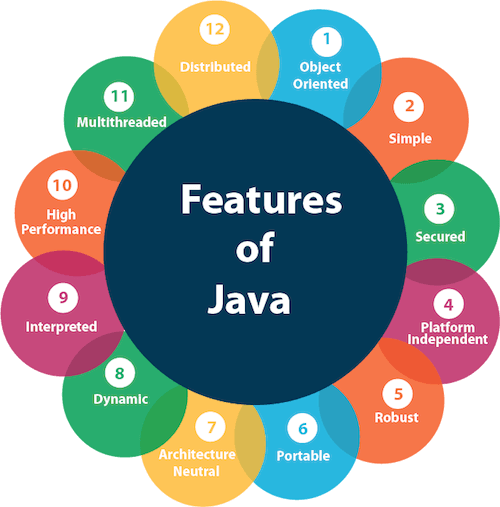
\includegraphics[width=78mm]{java-features.png}
\end{figure}
\end{frame}



\begin{frame}{First Java Program}
	\begin{itemize}
	\item  First Java Program Sample:	\end{itemize}
public class FirstProgram \{ \\

public static void main(String args[] ) \{ \\
  System.out.println("Helo World"); \\
\} \\
\} 
\item \textbf{Output}: \end{itemize}
    \textbf{javac FirstProgram.java\\
   java FirstProgram\\ 
Hello World}
\end{frame}


\begin{frame}{Key Point to remember}
	\begin{itemize}
	\item 	Case Sensitivity − Java is case sensitive, which means identifier Hello and hello would have different meaning in Java.


\item Class Names − For all class names the first letter should be in Upper Case. If several words are used to form a name of the class, each inner word's first letter should be in Upper Case.
		Example: class MyFirstJavaClass


\item Method Names − All method names should start with a Lower Case letter. If several words are used to form the name of the method, then each inner word's first letter should be in Upper Case.

		Example: public void myMethodName()


\item Program File Name − Name of the program file should exactly match the class name.


\item When saving the file, you should save it using the class name (Remember Java is case sensitive) and append '.java' to the end of the name (if the file name and the class name do not match, your program will not compile).

		Example: Assume 'FirstProgram' is the class name. Then the file should be saved as 'FirstProgram.java'


\item public static void main(String args[]) − Java program processing starts from the main() method which is a mandatory part of every Java program.


	\end{itemize}
\end{frame}



\begin{frame}{Popular Java Editors}
	\begin{itemize}
	\item All Java components require names. Names used for classes, variables, and methods are called identifiers.

\item In Java, there are several points to remember about identifiers. They are as follows:
					
\begin{itemize}
\item All identifiers should begin with a letter (A to Z or a to z), currency character (\$) or an underscore (\_).

	
\begin{itemize}
\item After the first character, identifiers can have any combination of characters.
\item A key word cannot be used as an identifier.
\item Most importantly, identifiers are case sensitive.
\end{itemize}
				Examples of legal identifiers: age, $salary, _value, __1_value.\\
					Examples of illegal identifiers: 123abc, -salary.
\end{itemize}
\end{itemize}
\end{frame}

\begin{frame}{Java Modifiers}
	\begin{itemize}
	\item 	
		Like other languages, it is possible to modify classes, methods, etc., by using modifiers. There are two categories of modifiers −
\item \textbf{Access Modifiers} − default, public , protected, private
\item \textbf{Non-access Modifiers }− final, abstract, strictfp

	\end{itemize}
\end{frame}

\begin{frame}{Java Keywords}
\begin{figure}[htpb]
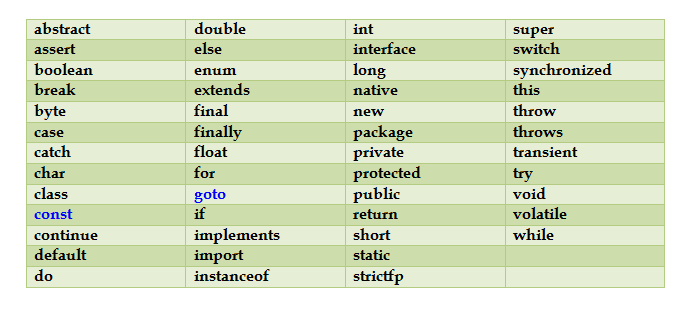
\includegraphics[width=125mm]{Java-Keywords.png}
\end{figure}\end{frame}


\begin{frame}{Comments in Java}
	\begin{itemize}
	\item 	
Java supports single-line and multi-line comments very similar to C and C++. All characters available inside any comment are ignored by Java compiler.\\
           \textbf{Example}  : \\ // Single line Comments. \\
                             /* Multi-line Comments. */ \\.	  
                             Documentation Comments(use for creating an API).

    
    \end{itemize}
\end{frame}

\end{document}

